\chapter{Non-parametric dynamic system using AIS tracking data}
On of the major issues with the direct approach is the unimodal assumption of using a \acrshort{gp}. This works well as long as vessels tends to agree on a specific trajectory, but fails as soon as there are multiple branching trajectories.

In \cite{pedestrian}, a \acrshort{gp} was used to model the trajectory patterns of pedestrians tracked using computer vision. Rather than directly describing trajectories, the paper proposed to simulate trajectories from a non-parametric dynamical model $\Delta\boldsymbol{x}_{t+1} = \vec{f}(\boldsymbol{x}_t)$ where the increments are expressed using a \acrshort{gp}. The trajectories were then simulated using two different approaches: 
\begin{enumerate}
    \item By assuming $p(\boldsymbol{x})$ is always uni-modal and Gaussian, the GP-EKF introduced in \cite{gpekf} was used to simulate the trajectory for multiple timesteps, using the dynamical \acrshort{gp} model as the prediction model. This formulation is unable to express multimodal uncertainty.
    \item In order to retain the inherent multimodality, a sequential Monte-Carlo approach (i.e. the prediction step of a particle filter) was used to keep track of multiple modes (i.e. branching trajectories), at the cost of computational complexity. 
\end{enumerate}

In this section, a similar method is proposed for long-term vessel prediction. The vessel trajectory $\boldsymbol{\mathcal{T}}$ can be expressed using the dynamical system
\begin{subequations}
\begin{align}
    \boldsymbol{x}_{t+1} &= \boldsymbol{x}_t + \vec{f}(\boldsymbol{x}_t)\\
    \mathcal{T}_t &= \boldsymbol{x}_t + \epsilon, \quad \epsilon \sim \mathcal{N}(0, \sigma^2)
\end{align}
\end{subequations}
The function $\vec{f}(\cdot): \mathcal{R}^2 \to \mathcal{R}^2$ denotes the vector field describing the expected velocity. In the case of long-term prediction, the dynamics $\vec{f}(\cdot)$ is unknown and is unlikely to be stationary. Instead of using the usual parametric approaches to ODE models, the goal of this chapter is to use a \acrshort{gp} to create a non-parametric representation of the dynamics $\vec{f}(\cdot)$ by learning from historical trajectories of other vessels. This way arbitrary complex dynamics can be learned, without being limited by the parametrization.

\begin{equation}\label{eq:gp_vec_field}
    \vec{f}(\boldsymbol{x}) = \begin{bmatrix} f_x (\boldsymbol{x})\\ f_y (\boldsymbol{x})\end{bmatrix} \sim \text{GP} \big(\begin{bmatrix} m_x(\boldsymbol{x})\\m_y(\boldsymbol{x})\end{bmatrix}, \ \begin{bmatrix}
    K_{xx}(\boldsymbol{x}, \boldsymbol{x}') & K_{xy}(\boldsymbol{x}, \boldsymbol{x}') \\ K_{xy}(\boldsymbol{x}, \boldsymbol{x}')^\intercal & K_{yy}(\boldsymbol{x}, \boldsymbol{x}')
    \end{bmatrix}\big) 
\end{equation}

The benefits of this formulation include:
\begin{description}
    \item[Easy incorporation of existing data] The model can easily be trained on partial data. Only the gradients of any historical trajectories are really needed.
    \item[Few constraining assumptions] The dynamical model is not constrained by any specific parametrization, while still allows prior knowledge such as smoothness to be incorporated into the model.
    \item[Branching trajectories] The dynamical formulation only assume Gaussian increments, while the full trajectory may still be multimodal. Though not analytically tractable, the multimodal trajectory can be found using sampling based methods. 
\end{description}

The major downside is however that the model only learns gradients from data and relies heavily on numerical simulations in order to get the desired trajectories.

The model could further be improved by clustering the samples based on similar behaviour for different ships, such as similar initial course and velocity. Separate \acrshort{gp}s could then be trained on the different subsets of data.

\section{Simulating trajectories using the Gaussian Process Extended Kalman Filter}
Once the dynamics $\vec{f}_*$ is conditioned on data, it can be used to predict trajectories using the prediction step from the \acrshort{ekf}. As the prediction $\vec{f}_*$ is non-linear, the Jacobian $\frac{\partial \vec{f}(\boldsymbol{x}_*)}{\partial \boldsymbol{x}_*}$ is necessary in order to calculate the predicted covariance in \acrshort{ekf} \cite{gpekf}. Luckily, since the derivative is a linear operator, calculating the Jacobian of $\vec{f}_*$ is simple, as derived in \cref{eq:gp_jacobian}. The \acrshort{ekf} prediction procedure in \cref{alg:gp_ekf_prediction} can then be called repeatedly to simulate the trajectory. 

\begin{align}\label{eq:gp_jacobian}
\begin{split}
    \frac{\partial \vec{f}(\boldsymbol{x}_*)}{\partial \boldsymbol{x}_*} &= \frac{\partial}{\partial \boldsymbol{x}_*} \bigg(\boldsymbol{k}_*^\intercal K^{-1} \big(\boldsymbol{y} - m(X)\big)\bigg)\\
    &= \frac{\partial \boldsymbol{k}_*^\intercal}{\partial \boldsymbol{x}_*} K^{-1} \big(\boldsymbol{y} - m(X)\big)\\ 
    &= \frac{\partial \boldsymbol{k}_*^\intercal}{\partial \boldsymbol{x}_*} \boldsymbol{\alpha} = \begin{bmatrix} 
    \frac{\partial k(\boldsymbol{x}_*, \boldsymbol{x}_1)}{\partial \boldsymbol{x}_*[1]} &  \frac{\partial k(\boldsymbol{x}_*, \boldsymbol{x}_1)}{\partial \boldsymbol{x}_*[2]} & \cdots & \frac{\partial k(\boldsymbol{x}_*, \boldsymbol{x}_1)}{\partial \boldsymbol{x}_*[M]} \\
    \frac{\partial k(\boldsymbol{x}_*, \boldsymbol{x}_2)}{\partial \boldsymbol{x}_*[1]} &  \frac{\partial k(\boldsymbol{x}_*, \boldsymbol{x}_2)}{\partial \boldsymbol{x}_*[2]} & \cdots & \frac{\partial k(\boldsymbol{x}_*, \boldsymbol{x}_2)}{\partial \boldsymbol{x}_*[M]} \\
    \vdots & \vdots & \ddots & \vdots\\
    \frac{\partial k(\boldsymbol{x}_*, \boldsymbol{x}_N)}{\partial \boldsymbol{x}_*[1]} &  \frac{\partial k(\boldsymbol{x}_*, \boldsymbol{x}_N)}{\partial \boldsymbol{x}_*[2]} & \cdots & \frac{\partial k(\boldsymbol{x}_*, \boldsymbol{x}_N)}{\partial \boldsymbol{x}_*[M]} \\
    \end{bmatrix}^\intercal \boldsymbol{\alpha}
\end{split}
\end{align}

\begin{algorithm}[h]
\begin{algorithmic}[1]
\Procedure{GP-EKF-PREDICT}{$\vec{f}$, $\boldsymbol{x}_{t-1}$, $\boldsymbol{P}_{t-1}$, $\Delta t$}
    \State $\boldsymbol{x}_{t} = \boldsymbol{x}_{t-1} + \vec{f}(\boldsymbol{x}_{t-1}) \Delta t$
    \State $\boldsymbol{F} = \frac{\partial \vec{f}(\boldsymbol{x}_{t-1})}{\partial \boldsymbol{x}_{t-1}} \Delta t$
    \State $\boldsymbol{P}_t = \boldsymbol{F}^\intercal \boldsymbol{P}_{t-1} \boldsymbol{F} +\mathbb{V}[\vec{f}(\boldsymbol{x}_{t-1})] (\Delta t)^2$
    \State \textbf{return} $\boldsymbol{x}_t, \; \boldsymbol{P}_t$
\EndProcedure
\end{algorithmic}
\caption{GP-EKF Trajectory Prediction}
\label{alg:gp_ekf_prediction}
\end{algorithm}

\begin{figure}
    \centering
    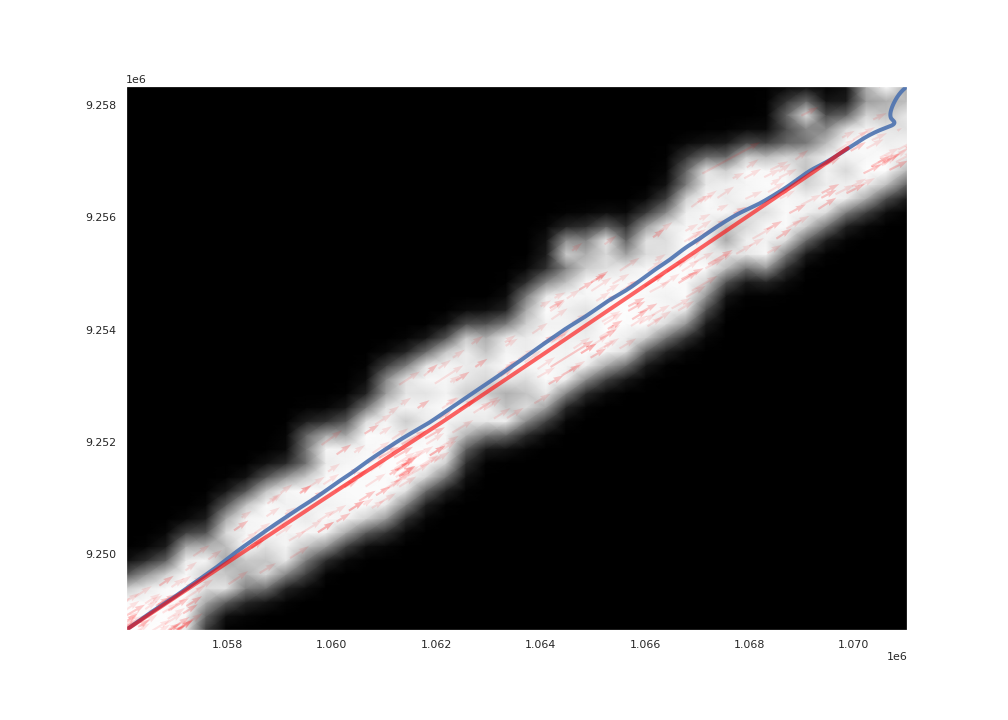
\includegraphics[width=\textwidth]{figures/gp_ekf.png}
    \caption{Placeholder figure}
    \label{fig:my_label}
\end{figure}

\begin{figure}
    \centering
    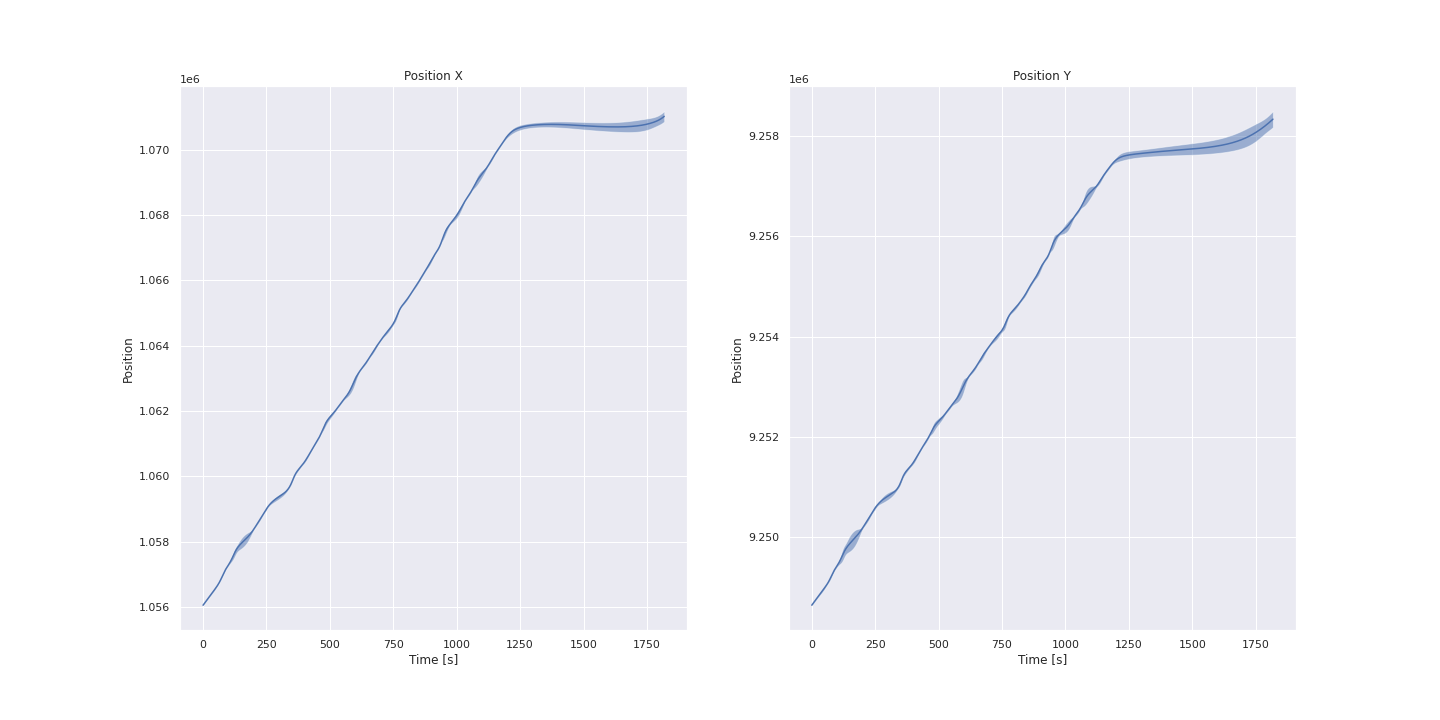
\includegraphics[width=\textwidth]{figures/gp_ekf_unc.png}
    \caption{Placeholder figure}
    \label{fig:my_label}
\end{figure}


\section{Simulating trajectories using Gaussian Process Sequential Monte Carlo}